\section{Optimizing Pointwise Convolution}
\label{sec:pwconv}
In this section, we demonstrate the workflow of our dynamic blocking strategy as shown in Figure \ref{fig:pwworkflow} and Algorithm \ref{algo:pwalgo}. 
The whole workflow consists of two stages. 

In the first stage, our approach operates in a top-down fashion. 
We use a 4-level hierarchical partitioning method to decompose the output into four levels of tiles, including SM level tiles, block level tiles, warp level tiles and thread level tiles. 
There are two main considerations when decomposing the output. First, how tiles are arranged in its upper level tile, and second, the height and width of each tile with the specified layout.

In the second stage, we calculate the exact height and width of thread level tiles. Given the number of output elements in each tile and hardware resources constraints, we iterate over all possible layout combinations of each level and choose the combination that maxmize the aritemetic intensity of a thread.

Now we give a detailed description of how each stage works.
\subsection{4-Level Hierarchical Partitioning}
In order to make it easier to understand the workflow of this stage, we first describe two important constant parameters and how we determine their values.

The first parameter is the number of warps in a thread block, denoted as $Warp_{num}$.
In order to determin the warp number, we need to consider: (1) small warp number will decrease the opportunity to hide the memory access latency at the warp level;
(2) large warp number will dcrease the number of thread blocks and may lead to SM underutilization.
Baed on both considerations, we decide to set $Warp_{num}=4$.
In our experiments, this value is good enough to provide a satisfied performance.

%this may not be important as i think
The second parameter is the number of thread blocks that can run concurrently in an SM, denoted as $Block_{num}$.
We use two values, 2, 4 and 6, for this parameter, denoted as $Block_{Num}=\{2, 4, 6\}$. 
There are two reasons for these choices: 
(1) when $Block_{num}=1$, there are only 4 warps in an SM. 
As each thread can use up to 256 registers, a thread block can use at most $4*32*256=32768$ registers, which is only 50\% of registers of an SM.
To avoid wasting hardware resources, we set $Block_{num}>1$; 
(2) when $Block_{num}>6$, each thread can use at most 70 registers and thus requires careful optimization on register usage to avoid register spills.
In our experiments, $Block_{num}=\{2, 4\}$ are the most commonly used values.

Now we demonstrate the workflow of 4-level hierarchical partitioning.
In our design, we can either distribute filter channels or input channels across threads. 
Therefore, we have two choices for the output layout and the corresponding logical views are shown in Figure \ref{fig:pwworkflow}.
For the output dimension that represents filter, we call it filter dimension, and the other one input dimension.
When partition the output into SM tiles, we always operate on the filter dimension and thus two layouts can share the same partition methods.
We design two partition methods, one divides the filter dimension into halves and the other keeps the filter dimension unchanged.
Once the partition method is decided, we can calculate the width of an SM tile in layout \textbf{\emph{L1}} with $SM_{W}=\{F_N/2,F_N\}$ and the height of an SM tile in layout \textbf{\emph{L2}} with $SM_{H}=\{F_N/2,F_N\}$.
In order to determine the size of the other dimension of an SM tile, we need to know the number of output elements in an SM tile.
When GPU is fully utilized, all $O_{size}$ output elements need to be distributed across all SMs, denoted as $SM_{num}$.
And the number of output elements in each SM tile is $SM_{size}=O_{size}/SM_{num}$.
Therefore, the height of an SM tile in layout \textbf{\emph{L1}} is $SM_{H}=SM_{size}/SM_W$ and the width of an SM tile in layout \textbf{\emph{L2}} is $SM_{W}=SM_{size}/SM_H$.

Now we get the height and width of an SM tile, {\color{red}the next step}is to partition the SM tile into block tiles.
We use the aforementationed partition method to divide the SM tile into block tiles, then the width of the block tile can be calculated as $Block_{W}=\{SM_W/2,SM_W\}$.
The heigh of the block tile will be determined in the second stage.
We use a fixed $2\times2$ layout to partition a block tile into 4 warp tiles, and the width of the warp tile is $Warp_{W}=Block_{W}/2$.
As mentioned earlier, each SM contains $Block_{num}$ thread blocks. 
We assume that each SM tile is divided into $Block_{num}$ block tiles, then the height of a block tile and a warp tile are $InitBlock_{H}=SM_{size}/Block_{num}/Block_{W}$ and $InitWarp_{H}=Block_{H}/2$ respectively. Since the height of block and warp tile can be modified, we label both notation with $Init$. 

\subsection{Distribute Channels Over Threads}
In this stage, we iterate over all candidate channel sizes and calculate two metrics for aritemetic intensity and thread block number with the constraints of register and shared memory.

To increase the arithmetic intensity, we need to distribute channels over threads. The most important cosideration is how to determine the number of threads that collaborate one output element. We use 6 values for the channel count, denoted as $C_{num}=\{1,2,4,8,16,32\}$. 
Figure \ref{fig:pwworkflow} demonstrates that we use 8 threads to calculate 8 channels of one output element at the same time. 

For each option of $C_{num}$, we calculate how many elements a warp can process at the same time, denoted as $Ele_{count}=32/C_{num}$. 
Then we get the number of elements each thread needs to process, denoted as $T_{num}=WarpTile_W/Ele_{count}$.
When calculating the same amount of output elements, square blocking uses the least load instructions. 
Therefore, we try to set the height of the thread tile to $T_{num}$.
First, we compare the value of $T_{num}$ with $InitWarp_H$.
If $T_{num}>InitWarp_H$, meaning there is not enough output elements to construct a square tile, we set $Warp_H=InitWarp_H$, otherwise, set $Warp_H=T_{num}$.
Then update $Block_H=2*Warp_H$.

Now we describe the constraints on registers and shared memory. Based on $Block_{num}$, we calculate the number of registers each thread can use and the size of shared memory each thread block can use, denoted as $Limit_R=65536/(Block_{num}*4*32)$ and $Limit_S=64*1024B/Block_{num}$ respectively.
The constraints can be formulated as follows:
\begin{equation}\nonumber
R_{o}=WarpTile_H*T_{num},R_{tmpf}=\frac{C_{num}*BlockTile_W}{128}
\end{equation}
\begin{equation}\nonumber
R_{f}=WarpTile_H,R_{i}=T_{num},R_{tmpi}=\frac{C_{num}*BlockTile_H}{128}
\end{equation}
\begin{equation}
R_{o}+R_{i}+R_{f}+R_{tmpf}+R_{tmpi}+const \leq Limit_R
\end{equation}
\begin{equation}
(BlockTile_H+BlockTile_W)*C_{num}*4*2 \leq Limit_S
\end{equation}
\begin{figure}
	\centering
    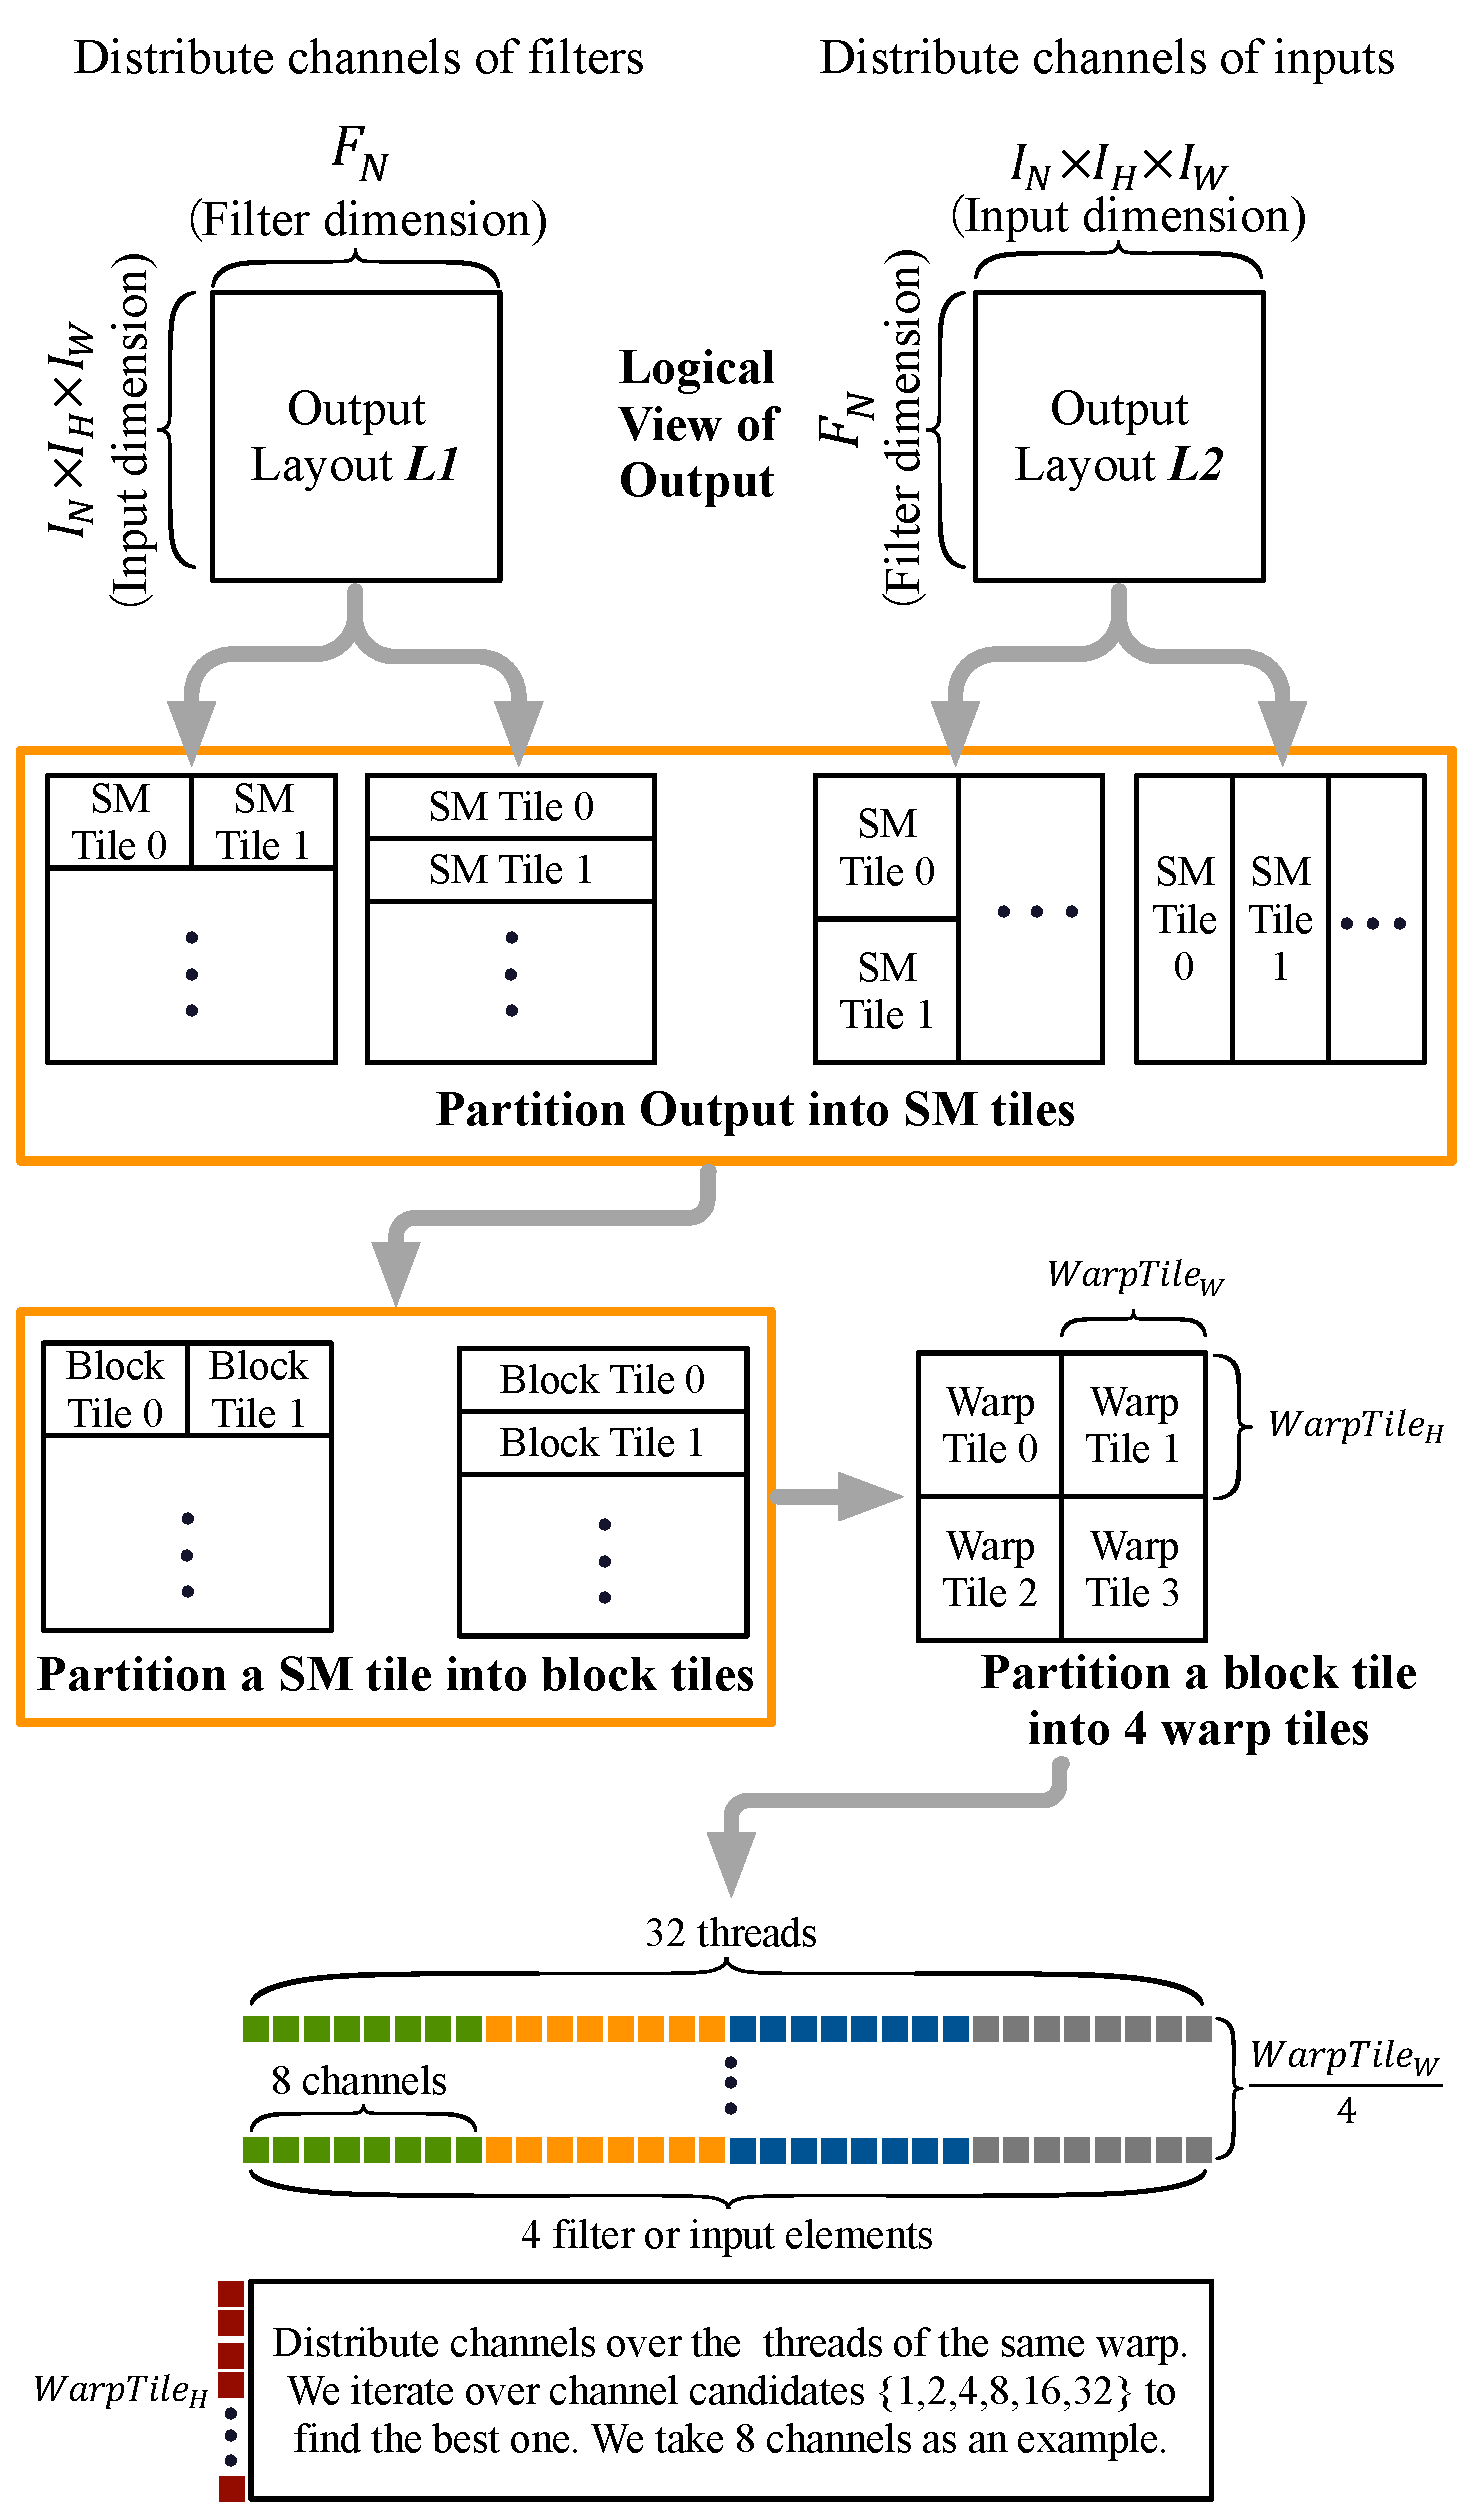
\includegraphics[width=\columnwidth]{./figure/pwworkflow.eps}
    \caption{} \label{fig:pwworkflow}
\end{figure}
\begin{algorithm}[t!]
    \small
        \KwIn{$I$, $F$}
        \KwOut{$O$}
        Calculate how many output elements one SM needs to process if we want to fully utilize GPU, denoted as $O_{sm}$\;
        \tcp{below codes are executed on CPU}
        \tcp{we have two options for block tile number, one SM contains 2 or 4 block tiles}
        \ForEach{block tile number of one SM}{
            Use $BlockTile_{count}$ to denote the number of block tiles resided on one SM\;
            \ForEach{block layout}{
                Calculate the width of a block tile, denoted as $BlockTile_W$\;
                $BlockTile_H = \frac{O_{sm}}{BlockTile_W * BlockTile_{count}}$\;
                \If{$BlockTile_H > 32$}{
                    $niter = BlockTile_H/32$\;
                    $BlockTile_H = 32$\;
                }
                $WarpTile_H=\frac{BlockTile_H}{2}$\;
                $WarpTile_W=\frac{BlockTile_W}{2}$\;
                \tcp{there are 6 choices for channel count, 1,2,4,8,16,32}
                \ForEach{channel count}{
                    Use $C_{count}$ to denote how many threads are uesed to calculate channels of the same output element.\;
                    $filter_{num} = \frac{32}{C_{count}}$\;
                    $filter_{num} = \frac{WarpTile_W}{filter_{num}}$\;
                    Calculate registers and shared memory usage under this configuration, and evaluate if the usage not exceeds the limit.\;
                    record the configuration with smallest register usage. 
                }
            }
        }
        \tcp{below codes are executed on GPU}
        All threads in a thread block cooperate to load the needed input and filter into shared memory\;
        $\_\_syncthreads()$\;
        \For{$iter \gets 0$ \KwTo $I_C$ By $C_{count}$}{
            load next $C_{count}$ channels for input and filter into registers\;
            load current channels of input and filter into registers\;
            calculate output elements\;
            write registers of next channels into shared memory\;
        }
        use segmented parallel reduce to get the final output elements and write the result to global memory\;
        \caption{Pointwise Convolution Optimization}
        \label{algo:pwalgo}
\end{algorithm}

We use two metrics, arithmetic intensity and thread block number, to select the best combinations. Two metrics are represented with notation $M_{A}$ and $M_{B}$, and can be calculated as follows:
\begin{equation}
    M_{A}=\frac{WarpTile_H*T_{num}*Iter}{R_{tmpf}+R_{tmpi}}
\end{equation}
\begin{equation}
    M_{B}=\frac{SM_H}{Block_H}*\frac{SM_W}{Block_W}*SM_{num}
\end{equation}

We first choose the best combination based on $M_{A}$, if two $M_{A}$ are close enough, then we choose the combination with smallest $M_{B}$. 